\documentclass[tikz,border=8pt]{standalone}
\usetikzlibrary{arrows.meta,calc}

\begin{document}
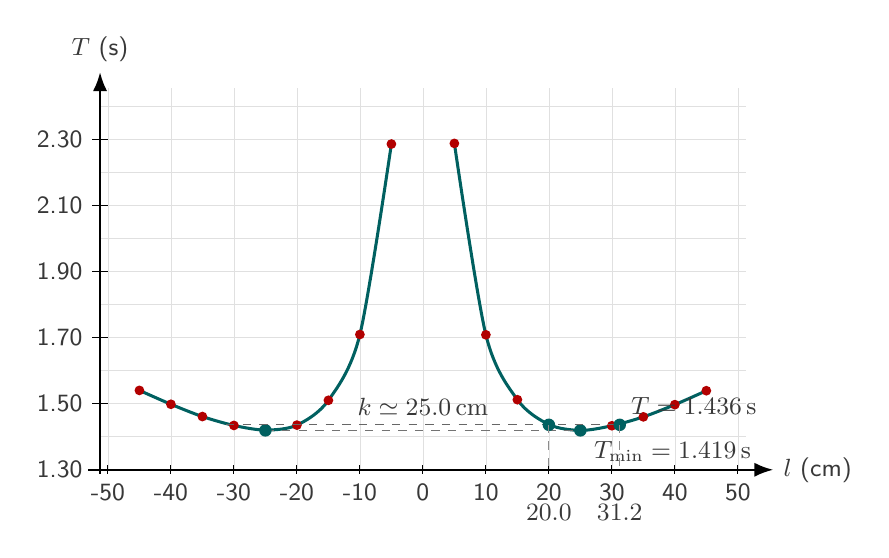
\begin{tikzpicture}[
  axis/.style={-{Latex[length=2.4mm]}, line width=0.8pt},
  grid/.style={line width=0.25pt, draw=black!12},
  curve/.style={line width=1.1pt, draw=teal!75!black},
  pointmark/.style={circle, fill=teal!75!black, inner sep=1.6pt},
  trial/.style={circle, fill=red!70!black, inner sep=1.25pt},
  note/.style={font=\sffamily\small, text=black!78},
]

% Coordinate system:
% x = 0.08 l, y = 4.2 (T - 1.30)

\draw[grid] (-4.1,0) grid[xstep=0.8,ystep=0.42] (4.1,4.85);
\draw[axis] (-4.25,0) -- (4.45,0) node[right, note] {$l$ (cm)};
\draw[axis] (-4.1,-0.05) -- (-4.1,5.05) node[above, note] {$T$ (s)};

% x ticks
\foreach \x/\lab in {-4/-50,-3.2/-40,-2.4/-30,-1.6/-20,-0.8/-10,0/0,0.8/10,1.6/20,2.4/30,3.2/40,4/50} {
  \draw (\x,0.06) -- (\x,-0.06) node[below, note] {\lab};
}

% y ticks
\foreach \y/\lab in {0/1.30,0.84/1.50,1.68/1.70,2.52/1.90,3.36/2.10,4.20/2.30} {
  \draw (-4.0,\y) -- (-4.2,\y) node[left, note] {\lab};
}

% Left and right branches from trial data
\draw[curve, smooth]
  plot coordinates {(-3.6,1.008) (-3.2,0.832) (-2.8,0.676) (-2.4,0.563) (-2.0,0.504) (-1.6,0.567) (-1.2,0.882) (-0.8,1.718) (-0.4,4.137)};
\draw[curve, smooth]
  plot coordinates {(0.4,4.145) (0.8,1.714) (1.2,0.890) (1.6,0.575) (2.0,0.500) (2.4,0.559) (2.8,0.672) (3.2,0.827) (3.6,1.004)};

% Trial points
\foreach \x/\y in {
  -3.6/1.008,-3.2/0.832,-2.8/0.676,-2.4/0.563,-2.0/0.504,-1.6/0.567,-1.2/0.882,-0.8/1.718,-0.4/4.137,
  0.4/4.145,0.8/1.714,1.2/0.890,1.6/0.575,2.0/0.500,2.4/0.559,2.8/0.672,3.2/0.827,3.6/1.004
} {
  \node[trial] at (\x,\y) {};
}

% Mark minimum and working horizontal line
\draw[black!55, dashed] (-2.0,0.50) -- (2.0,0.50);
\node[pointmark] at (2.0,0.50) {};
\node[pointmark] at (-2.0,0.50) {};
\node[note, below right] at (2.05,0.48) {$T_{\min}=1.419\,\mathrm{s}$};
\node[note, above] at (0,0.56) {$k\simeq 25.0\,\mathrm{cm}$};

\draw[black!60, dashed] (-2.50,0.571) -- (2.50,0.571);
\node[pointmark] at (1.60,0.571) {};
\node[pointmark] at (2.50,0.571) {};
\draw[black!45, dashed] (1.60,0.571) -- (1.60,0);
\draw[black!45, dashed] (2.50,0.571) -- (2.50,0);
\node[note, above right] at (2.52,0.58) {$T=1.436\,\mathrm{s}$};
\node[note, below] at (1.60,-0.32) {$20.0$};
\node[note, below] at (2.50,-0.32) {$31.2$};

\end{tikzpicture}
\end{document}
